\documentclass{elsarticle}




\usepackage[dvipsnames]{xcolor}
\usepackage[backgroundcolor=magenta!10!white]{todonotes}

\usepackage{microtype}


\usepackage{amsmath,amssymb,amsfonts}

\usepackage{graphicx}





\usepackage{ifthen}

\usepackage{numprint}
\npdecimalsign{.}
\npthousandsep{,}

\usepackage{hyperref}


\usepackage{thm-restate}

\usepackage{tikz}
\usetikzlibrary{arrows,
automata,
calc,
decorations,
decorations.pathreplacing,
positioning,
shapes}







\newtheorem{definition}{Definition}
\newtheorem{theorem}[definition]{Theorem}
\newtheorem{lemma}[definition]{Lemma}
\newtheorem{proposition}[definition]{Proposition}
\newtheorem{corollary}[definition]{Corollary}
\newtheorem{example}[definition]{Example}
\newtheorem{remark}{Remark}[section]
\newtheorem{notation}[definition]{Notation}
\newtheorem{fact}[definition]{Fact}
\newproof{proof}{Proof}




\usepackage{caption}
\captionsetup[table]{skip=10pt}
\usepackage{lscape}


 




\newcommand{\barQ}{\overline{Q}}
\newcommand{\barn}{\overline{n}}





\def\Ende{\hfill {\tiny }}




\def\eqdef{\stackrel{\text{def}}{=}}

\def\<{\langle}
\def\>{\rangle}




\def\Nat{\mathbb{N}}
\def\Integer{\mathbb{Z}}
\def\Real{\mathbb{R}}
\def\Rational{\mathbb{Q}}




\def\cA{\mathcal{A}}
\def\cB{\mathcal{B}}
\def\cC{\mathcal{C}}
\def\cD{\mathcal{D}}
\def\cE{\mathcal{E}}
\def\cF{\mathcal{F}}
\def\cG{\mathcal{G}}
\def\cH{\mathcal{H}}
\def\cI{\mathcal{I}}
\def\cJ{\mathcal{J}}
\def\cK{\mathcal{K}}
\def\cL{\mathcal{L}}
\def\cM{\mathcal{M}}
\def\cN{\mathcal{N}}
\def\cO{\mathcal{O}}
\def\cP{\mathcal{P}}
\def\cQ{\mathcal{Q}}
\def\cR{\mathcal{R}}
\def\cS{\mathcal{S}}
\def\cT{\mathcal{T}}
\def\cU{\mathcal{U}}
\def\cV{\mathcal{V}}
\def\cW{\mathcal{W}}
\def\cX{\mathcal{X}}
\def\cY{\mathcal{Y}}
\def\cZ{\mathcal{Z}}





\def\fA{\mathfrak{A}}
\def\fB{\mathfrak{B}}
\def\fC{\mathfrak{C}}
\def\fD{\mathfrak{D}}
\def\fE{\mathfrak{E}}
\def\fF{\mathfrak{F}}
\def\fG{\mathfrak{G}}
\def\fH{\mathfrak{H}}
\def\fI{\mathfrak{I}}
\def\fJ{\mathfrak{J}}
\def\fK{\mathfrak{K}}
\def\fL{\mathfrak{L}}
\def\fM{\mathfrak{M}}
\def\fN{\mathfrak{N}}
\def\fO{\mathfrak{O}}
\def\fP{\mathfrak{P}}
\def\fQ{\mathfrak{Q}}
\def\fR{\mathfrak{R}}
\def\fS{\mathfrak{S}}
\def\fT{\mathfrak{T}}
\def\fU{\mathfrak{U}}
\def\fV{\mathfrak{V}}
\def\fW{\mathfrak{W}}
\def\fX{\mathfrak{X}}
\def\fY{\mathfrak{Y}}
\def\fZ{\mathfrak{Z}}







\newcommand{\PTIME}{\mathrm{P}}
\newcommand{\NP}{\mathrm{NP}}
\newcommand{\coNP}{\mathrm{coNP}}
\newcommand{\PSPACE}{\mathrm{PSPACE}}
\newcommand{\EXPTIME}{\mathrm{EXPTIME}}







\def\Pr{\mathrm{Pr}}

\def\Paths{\mathit{Paths}}
\def\Act{\mathit{Act}}
\def\AP{\mathit{AP}}
\def\Acc{\mathit{Acc}}
\def\accEC{\mathit{accEC}}
\def\trace{\mathit{trace}}
\def\lab{\mathit{lab}}
\def\Post{\mathrm{Post}}

\def\qinit{q_{\textit{\tiny init}}}
\def\qtrap{q_{\textit{\tiny trap}}}
\def\qfinal{q_{\textit{\tiny final}}}

\def\qfinal{\mathit{final}}

\def\QSCC{Q_{\mathit{SCC}}^{>0}}
\def\QBSCC{Q_{\mathit{BSCC}}}
\def\Qunknown{Q_{?}}

\newcommand{\scc}[1]{\cC_{#1}}

\def\trace{\mathit{trace}}
\def\accrun{\mathit{accrun}}
\def\Runs{\mathit{Runs}}
\def\Pref{\mathit{Pref}}

\newcommand{\SCC}[1]{\mathit{SCC}(#1)}

\def\Cyl{\mathit{Cyl}}

\def\first{\mathit{first}}
\def\last{\mathit{last}}

\def\infoften{\mathit{inf}}

\def\cLomega{\cL_{\omega}}
\def\cLfin{\cL_{\textit{\tiny fin}}}

\def\sched{\mathfrak{S}}

  
\newcommand{\move}[1]{\stackrel{#1}{\longrightarrow}}

\newcommand{\sroot}[1]{\mathit{root}(#1)}

\newcommand{\notapplicable}{}
\newcommand{\subpointone}{\,}




\newcommand{\extended}[1]{\hat{#1}}
\newcommand{\detlim}[1]{#1_{\text{\tiny \rm detlim}}}
\newcommand{\Det}[1]{#1_{\text{\tiny \rm det}}}

\newcommand{\NFA}[1]{#1_{\text{\tiny \rm NFA}}^{\text{\tiny all}}}

\newcommand{\Mon}{\mathit{Mon}}






\newcommand{\until}{\cU}
\newcommand{\finally}{\Diamond}
\newcommand{\globally}{\Box}
\newcommand{\neXt}{\bigcirc}



\newcommand{\psec}[1]{\nprounddigits{1}\npfourdigitnosep\numprint[s]{#1}}
\newcommand{\pnodes}[1]{\nprounddigits{0}\numprint{#1}}



\newcommand{\prism}{\texttt{PRISM}}
\newcommand{\colt}{\texttt{COLT}}
\newcommand{\spot}{\texttt{SPOT}}
\newcommand{\ltltodstar}{\texttt{ltl2dstar}}
\newcommand{\ltltotgba}{\texttt{ltl2tgba}}
\newcommand{\rabinizer}{\texttt{Rabinizer}}
\newcommand{\tulip}{\texttt{Tulip}}
\newcommand{\iscasmc}{\texttt{IscasMC}}
\newcommand{\delag}{\texttt{Delag}}

\newcommand{\explicitengine}{\texttt{explicit}}





\newcommand{\todowithauthor}[4]{\todo[linecolor=gray,backgroundcolor=#3, #1]{#2\hfill{\scriptsize{\em{#4}}}}}

\colorlet{davidColor}{YellowGreen!30!white}
\colorlet{stefanColor}{Brown!30!white}
\colorlet{benColor}{Yellow!30!white}


\newcommand{\todoDavid}[2][]{\todowithauthor{#1}{#2}{davidColor}{David}}


\newcommand{\todoStefan}[2][]{\todowithauthor{#1}{#2}{stefanColor}{Stefan}}
\newcommand{\todoBen}[2][]{\todowithauthor{#1}{#2}{benColor}{Ben}}


\newcommand{\vzero}{\vec{0}}\newcommand{\vone}{\vec{1}}\newcommand{\tB}{\overline{B}}
\newcommand{\rank}{\mathrm{rank}}





 
\sloppy

\newcommand{\Ex}{\mathrm{Ex}}
\newcommand{\then}{\mathord{\triangleright}}

\begin{document}
\begin{abstract}
  Unambiguous automata are nondeterministic automata in which every
  word has at most one accepting run.  In this paper we give a
  polynomial-time algorithm for model checking discrete-time Markov
  chains against -regular specifications represented as unambiguous
  automata.  We furthermore show that the complexity of this model
  checking problem lies in NC: the subclass of P comprising
  those problems solvable in poly-logarithmic parallel time.  These
  complexity bounds match the known bounds for model checking Markov
  chains against specifications given as deterministic automata,
  notwithstanding the fact that unambiguous automata can be
  exponentially more succinct than deterministic automata.  We report
  on an implementation of our procedure, including an experiment in
  which the implementation is used to model check LTL formulas on
  Markov chains.
\end{abstract}
\pagestyle{headings}  

\title{Markov Chains and Unambiguous Automata}


\author[tud]{Christel Baier\texorpdfstring{\fnref{tudthanks}}{}}
\author[oxf]{Stefan Kiefer\texorpdfstring{\fnref{kieferthanks}}{}}
\author[tud]{Joachim Klein\texorpdfstring{\fnref{tudthanks}}{}}
\author[tud]{David M\"uller\texorpdfstring{\fnref{tudthanks}}{}}
\author[oxf]{James Worrell\texorpdfstring{\fnref{worrellthanks}}{}}





\address[tud]{Technische Universit\"at Dresden, Germany}
\address[oxf]{University of Oxford, United Kingdom}
\fntext[tudthanks]{The authors are supported by the DFG through
        the Collaborative Research Center 
        TRR 248 (see \url{https://perspicuous-computing.science}, project ID 389792660),
        the DFG project BA-1679/12-1,
        the Cluster of Excellence EXC 2050/1 (CeTI, project ID 390696704, as part of Germany's Excellence Strategy), and
        the Research Training Group QuantLA (GRK 1763). }
\fntext[kieferthanks]{Kiefer is supported by a University Research Fellowship of the Royal Society.}
\fntext[worrellthanks]{Worrell is supported by EPSRC grant EP/M012298/1.}
\maketitle              


 
\section{Introduction}

Unambiguity is a generalization of determinism that has been widely
studied in the theory and applications of
automata~\cite{Colcombet12,Colcombet15}.  In this paper we are
concerned with unambiguous automata over infinite words, that is,
nondeterministic automata in which every word has at most one
accepting run.  Our main results hold for the most commonly occurring
acceptance conditions (B\"{u}chi, Rabin, Muller, etc.), however in our
examples and experimental results we focus on the case of unambiguous
B\"{u}chi automata (UBA).  An example of a UBA is the automaton on the
right-hand side of Fig.~\ref{fig:uba-examples} in which both states
are initial and accepting.  This automaton is unambiguous by virtue of
the fact that there is exactly one run over every word.


Over infinite words, not only are UBA as expressive as
nondeterministic B\"uchi automata~\cite{Arnold85}, they can also be
exponentially more succinct than deterministic automata.  For example,
for a fixed 
the language ``eventually  occurs and  appears  steps before
the first '' over the alphabet  is recognized by a UBA
with  states (shown on the left-hand side of
Figure~\ref{fig:uba-examples}).  On the other hand, a deterministic
automaton for this language requires at least  states, regardless
of the acceptance condition, as it needs to store the positions of the
's among the last  input symbols.  Languages of this type arise
in a number of contexts, e.g., absence of unsolicited response in a
communication protocol---if a message is received, then it has been
sent in the recent past.

\begin{figure}[tbp]
\begin{minipage}{0.64\textwidth}\begin{tikzpicture}[initial text=, initial where=above, node distance= 0.18 \textwidth, scale=0.95, every node/.style={semithick, scale=0.95}, every path/.style={semithick, scale=0.95}]
    \node[state, ellipse, initial, minimum size=5 ex, inner sep=0.5 ex]  (q0)                        {};
    \node[state, ellipse, minimum size=5 ex, inner sep=0.5 ex]           (qa)    [right of=q0]       {};
    \node[state, ellipse, minimum size=5 ex, inner sep=0.5 ex, align=center]           (q1)    [right of=qa]       {};
    \node[state, ellipse, minimum size=5 ex, inner sep=0 ex, align=center]           (q2)    [right of=q1]       {};
    \node[align=center,draw=none]   (cdots) at()   {};
    \node[state, ellipse, minimum size=5 ex, inner sep=0 ex]           (q3)    [right of=q2]       {};
    \node[state, ellipse, accepting, minimum size=5 ex, inner sep=0.5 ex]           (qf)    [right of=q3]       {};

    \draw[->]   (q0)    edge[loop below]     node[below]    {}  (q0);
    \draw[->]   (q0)    edge[]               node[above]    {}  (qa);
    \draw[->]   (qa)    edge[]               node[above]    {}  (q1);
    \draw[->]   (q2)    edge[]               node[above]    {}  (q3);
    \draw[->]   (q3)    edge[]               node[above]    {}  (qf);
    \draw[->]   (qf)    edge[loop below]     node[below]    {}  (qf);

    \draw[decorate,decoration={brace, mirror, amplitude=2 ex, raise=0.8 ex}, semithick] (qa.south) -- node[below, yshift=-3 ex] { steps} (q3.south);
\end{tikzpicture}\end{minipage}\begin{minipage}{0.35\textwidth}\raggedleft
\hspace*{1 ex}
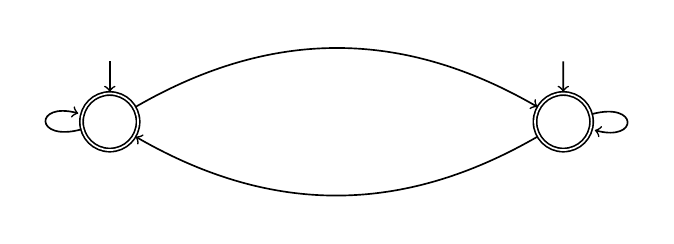
\begin{tikzpicture}[initial text=, initial where=above, node distance= 0.5 \textwidth, scale=0.95, every node/.style={semithick, scale=0.95}, every path/.style={semithick, scale=0.95}]
    \node[state, ellipse, initial, minimum size=5 ex, inner sep=0.5 ex, accepting]  (qa)                 {};
    \node[state, ellipse, initial, minimum size=5 ex, inner sep=0.5 ex, accepting]  (qb) [right of=qa]   {};

    \draw[->]   (qa)    edge[loop left]     node[left]    {}  (qa);
    \draw[->]   (qa)    edge[bend left]     node[above]   {}  (qb);
    \draw[->]   (qb)    edge[loop right]    node[right]   {}  (qa);
    \draw[->]   (qb)    edge[bend left]     node[below]   {}  (qa);
\end{tikzpicture}
\end{minipage}\caption{Left: UBA for ``eventually  and  appears  steps before first
'', right: A universal and separated UBA.}
\label{fig:uba-examples}
\end{figure}





The exponential succinctness of UBA relative to deterministic automata
is also manifested in translations of linear temporal logic
(LTL) to automata.  The nondeterministic B\"{u}chi automata that are
obtained from LTL formulas by applying the classical closure algorithm
of~\cite{WVS83,VardiWolper86} are unambiguous. The generated automata
moreover enjoy the separation property: different states
have disjoint languages.  Thus, while the generation of deterministic
-automata from LTL formulas incurs a double-exponential
blow-up in the worst case, the translation of LTL formulas into
separated UBA incurs only a single exponential blow-up. This fact has
been observed by several authors, see
e.g.~\cite{CouSahSut03,MorgensternThesis}, and adapted for LTL with
step parameters~\cite{Zimmermann13,ChaKat14}.
Besides allowing exactly one accepting run for every accepted word, there exist
weaker notions of unambiguity, where one allows a finite number of runs, or a
polynomial number of runs~\cite{RI89,HSS17}. These forms of unambiguity led to applications in
complementation of B\"uchi automata with a finite number of accepting runs~\cite{Rabinovich18}.



In the context of probabilistic model checking, UBA provide an elegant
alternative to deterministic automata for computing probabilities of
-regular properties on finite-state Markov chains.  A
polynomial-time model checking procedure for UBA that represent safety
properties was given~\cite{BenLenWor14}, while~\cite{CouSahSut03}
gives a polynomial-time algorithm for separated UBA.  However,
separation is a strong restriction, as non-separated UBA (and even
DBA) can be exponentially more succinct than separated UBA,
see~\cite{BousLoed10}.  Furthermore, algorithms for the generation of
(possibly non-separated) UBA from LTL formulas that are more compact
than the separated UBA generated by the classical closure algorithm
have been realized in the tool \tulip{}
\cite{LenhardtThesis13,Len-Tulip13} and the automata library
\spot{}~\cite{Duret13}.  This motivates the design of algorithms that
operate with general UBA rather than the subclass of separated UBA.
For the analysis of finite-state Markov decision processes under
-regular properties, there exist restricted forms of
nondeterministic automata such as limit-deterministic automata
\cite{Vardi85,CY95,SEJK16} or good-for-games automata
\cite{HP06,KMBK14}.

The main theoretical contribution of this paper is a polynomial-time
algorithm to compute the probability that the trajectory generated by
a given finite Markov chain satisfies an -regular property
specified by a (not necessarily separated) unambiguous automaton.  We
present this algorithm under a mild assumption on the acceptance
condition of the automaton, which is satisfied by commonly occurring
acceptance conditions such as B\"{u}chi, Rabin, Muller, etc.
Furthermore we use our procedure to show that the model checking
problem of finite Markov chains against unambiguous automata lies in
the complexity class NC: the subclass of P comprising those problems
solvable in poly-logarithmic time by a parallel random-access machine
using polynomially many processors.

The existence of a polynomial-time algorithm for model checking Markov
chains against UBA has previously been claimed
in~\cite{BenLenWor13,BenLenWor14,LenhardtThesis13} (see
also~\cite{Len-Tulip13}).  However, these previous works share a
common fundamental error.  Specifically they rely on the claim that if
the language of a given UBA  has positive probability with
respect to a Markov chain , then there exists a state  of
 and a state  of  such that  accepts almost all
trajectories emanating from  (see~\cite[Lemma
7.1]{BenLenWor13},~\cite[Theorem 2]{BenLenWor14}\footnote{As the flaw is in the handling of the infinite behavior, the
  claim and proof of Lemma~1 in~\cite{BenLenWor14}, dealing with
  unambiguous automata over finite words, remain unaffected.  }
and~\cite[Section 3.3.1]{LenhardtThesis13}).  While this claim is true
in case  is deterministic~\cite{CY95}, it need not hold when
 is merely unambiguous (see
Remark~\ref{rem:counter-example-uba}).  We refer the reader
to~\cite{BKKKMW16} for full details and counterexamples to incorrect
claims in these works.

As a corollary of the above-mentioned NC bound we obtain another proof
of the fact that model checking LTL formulas on Markov chains can be
done in polynomial space (see~\cite{BusRubVar04} for a proof of this
fact using weak alternating automata and see~\cite{CY88,CY95} for an
automata-free approach).  Another corollary of our main result is that
one can decide in NC whether a given UBA accepts almost all words with
respect to the uniform distribution on -words.  Recall that
while checking universality is known to be in NC for
deterministic B\"uchi automata and PSPACE-complete for NBA,
determining the complexity of the universality problem for UBA is a
long-standing open problem.  Polynomial-time procedures are only known
for separated UBA and other subclasses of
UBA~\cite{BousLoed10,IsaLoed12}.



A second contribution of our paper is an implementation of the new
algorithm as an extension of the model checker \prism{}, using the
automata library \spot{}~\cite{Duret13} for the generation of UBA from
LTL formulas and the \colt{} library~\cite{Hoschek04} for various
linear algebra algorithms.
We focus on unambiguous automata with a B\"uchi acceptance condition.
We evaluate our approach using the bounded
retransmission protocol case study from the PRISM benchmark suite
\cite{prismBenchmark} as well as specific aspects of our algorithm
using particularly ``challenging'' UBA.

We remark that there cannot exist a polynomial-time algorithm for model checking Markov decision processes (MDPs) against UBA.
This is because model checking LTL formulas on MDPs is 2EXPTIME-complete~\cite{CY95} and there is a single-exponential procedure for translating LTL formulas into UBA (cf.\ the proof of Corollary~\ref{cor:LTL-PSPACE}).

The rest of this article is structured as follows.
In Section~\ref{sec:prelim} we provide the necessary definitions and quote standard results on the spectral theory of nonnegative matrices.
In Section~\ref{sec:overview} we give an overview of our methodology.
Section~\ref{sec:uba} contains the main technical development with a polynomial-time model checking procedure.
Key technical lemmas are proved in Sections \ref{sec:recurrent-proof} and~\ref{sec:cut-proof}.
Section~\ref{sec:NC} improves the main result to an NC model checking procedure.
In Section~\ref{uba_implementation} we describe our implementation and experiments.
We conclude in Section~\ref{sec:conclusion}.

This article is a revised version of the CAV'16 conference
paper~\cite{BKKKMW16} and its extended version on
arxiv~\cite{cav16full}.  The main differences are that we present here
a direct proof technique, while \cite{BKKKMW16,cav16full} first
explain how to compute the measure of the language induced by strongly
connected UBA and then how to extend these techniques to arbitrary UBA
and the probabilistic model checking problem as discussed here.  In
contrast to \cite{BKKKMW16,cav16full} we consider here acceptance
conditions beyond B\"uchi acceptance.  Furthermore, the material on
experiments has been extended.

\section{Preliminaries}
\label{sec:prelim}

We assume the reader to be familiar with basic notions of Markov
chains and finite automata over infinite words, see, e.g., \cite{GraedelThomasWilke02,Kulkarni} and complexity theory, see, e.g., \cite{Pap94}.  In what follows, we
provide a brief summary of our notation for words, finite automata,
vectors and matrices, and Markov chains.
We also briefly summarize basic facts on the complexity class~NC and collect facts in the spectral theory of nonnegative matrices.

\paragraph*{Words}
Throughout the article, we suppose that  is a finite non-empty alphabet.
For  and  we write  for the concatenation of  and~, i.e., .
If  for some  then we may write  for .

\paragraph*{Finite automata}
A (nondeterministic finite) automaton (over infinite words)
is a tuple 
where  is the finite set of states,  is the set of initial
states,  is the alphabet,
 is
the transition function, and  is the (Muller) acceptance condition.
We extend the transition function to 
and to  in the standard way.
Given states  and a finite word
,
a \emph{run} for  from  to  is a sequence
 with ,  and
 for .
A \emph{run} in  for an infinite word
 is an infinite sequence
 such that  and
 for all .  Run  is
called \emph{accepting} if  where
 is the set of states that occur infinitely
often in~.  The \emph{language}  of accepted words
consists of all infinite words  that have at
least one accepting run.
If  then  denotes the automaton  with 
as set of initial states.  If  is understood from the context and
 then we may write  for~.
 is called  \emph{deterministic} if  is a singleton and    for all  and , and \emph{unambiguous} if each word  has at most one accepting run in~.
Clearly, each deterministic automaton is unambiguous.

We assume that, given any set , one can compute in
polynomial time whether .  This is the case, e.g., if
 is given as a \emph{B\"uchi} condition, i.e., as a set
 of \emph{accepting} states such that  if
and only if .
We use the acronym UBA for unambiguous B\"uchi automata.

We say that an automaton~ has a \emph{diamond} from  to~
(where ) if there is a finite word  such
that there are at least two different runs for~ from  to~.
If  has no diamonds, we say that  is \emph{diamond-free}.
If  is an unambiguous automaton then one can make it diamond-free
in polynomial time and even in~NC: First remove all states that are unreachable
from~, along with their incoming and outgoing transitions.  Then
compute, in polynomial time, all states  such that there is a
diamond from  to~.  By unambiguousness, we have
, so we can remove~ from~, along with all
incoming and outgoing transitions, without changing .
Therefore we can and will generally assume that unambiguous automata are diamond-free.

\paragraph*{Complexity Theory}

Let  be a family of Boolean circuits such
that  has  input gates and any number of output gates.  Such a
family is said to be \emph{uniform} if there is a -space
bounded Turing machine which on input  outputs .  Such a
family is moreover said to compute a function
 if for each  and
every word  the output of  on input  equals
.
Function~ is said to be computable in NC if there exists a
positive integer  such that  is computed by a uniform family
of circuits  where  has depth
.  NC is widely considered as the subclass of
polynomial-time computable functions comprising those functions that
can be computed efficiently (i.e., in poly-logarithmic time) in
parallel (see, e.g.,~\cite[Chapter 15]{Pap94}).

A standard result of complexity theory is that a function computable
in NC is computable by a Turing machine using poly-logarithmic
space~\cite[Theorem 4]{Borodin77}.  Two facts that will be used below
are that reachability in directed graphs and matrix determinants (and
hence solving systems of linear equations) are both computable in
NC~\cite{Pap94}.

\paragraph*{Vectors and matrices}
We consider vectors and square matrices indexed by a finite set~.
We use boldface for (column) vectors such as ,
and write  for the transpose (a row vector)
of~.  The zero vector and the all-ones vector are denoted
by~ and , respectively.  A matrix
 is called \emph{stochastic} if
, i.e., if every row of  sums to one.  For a
set  we write  for the
restriction of~ to~.  Similarly, for  we
write  for the submatrix of~ obtained by deleting the rows
not indexed by~ and the columns not indexed by~.  The (directed)
\emph{graph} of a nonnegative matrix  has
vertices  and edges  if .  We may
implicitly associate~ with its graph and speak about
graph-theoretic concepts such as reachability and strongly connected
components (SCCs) in~.  For  we write
,
, and
.





\paragraph*{Markov chains}
A (finite-state discrete-time) \emph{Markov chain} is a pair
 where  is the finite set of states, and
 is a stochastic matrix that specifies
transition probabilities.  An \emph{initial distribution} is a
function  satisfying
.  Such a distribution induces a
probability measure~ on the measurable subsets
of~ in the standard way.
We may write  for~ if  is understood.
If  is concentrated on a
single state~ then we may write 
for~.  Note that
.

\paragraph*{Spectral Theory}
The \emph{spectral radius} of a matrix ,
denoted , is the largest absolute value of the eigenvalues
of~.  The following result summarizes some facts in the spectral
theory of nonnegative matrices that will be used in the sequel.
In the
formulation below, we restrict attention to right eigenvectors.


\begin{theorem}
  Let  be a nonnegative matrix.  Then
  the following all hold:
\begin{enumerate}
\item The spectral radius  is an eigenvalue of~ and there
  is a nonnegative eigenvector  with
  .
  Such a vector~ is called \emph{dominant}.
\item If  then .
\item There is  such that  is strongly connected and .
\end{enumerate}
\label{thm:nonnegative}
\end{theorem}

\begin{theorem}
  Let  be a strongly connected nonnegative
  matrix.  We have the following facts:
\begin{enumerate}
\item There is an eigenvector  with
   such that  is
  strictly positive in all components.
\item The eigenspace associated with  is one-dimensional.
\item If  then .
\item If  and  
then .
\item If  is strictly positive, i.e.,  for all , then  exists and is strictly positive.
\end{enumerate}
\label{thm:irreducible}
\end{theorem}

These results can mostly be found in~\cite[Chapter 2]{book:BermanP94}.
Specifically, Theorems \ref{thm:nonnegative}(1) and \ref{thm:irreducible}(1--2) are part of the Perron-Frobenius theorem, see \cite[Theorems 2.1.1, 2.1.4]{book:BermanP94};
Theorem~\ref{thm:nonnegative}(2) is \cite[Corollary 2.1.6(a)]{book:BermanP94};
Theorem~\ref{thm:nonnegative}(3) follows from \cite[Corollary 2.1.6(b)]{book:BermanP94};
Theorem~\ref{thm:irreducible}(3) follows from \cite[Corollary 2.1.6]{book:BermanP94};
Theorem~\ref{thm:irreducible}(4) follows from \cite[Corollary 2.1.11]{book:BermanP94};
Theorem~\ref{thm:irreducible}(5) follows from \cite[Theorem 8.2.7]{HornJohnson13}.


\section{Overview of the Methodology} \label{sec:overview}

Given a finite Markov chain  and an unambiguous automaton ,
our goal is to compute the probability that a trajectory
generated by  is accepted by~ for a given initial distribution~.  Suppose that  has set
of states  and  has set of states .  Let vector
 be such that for each 
and ,  is the probability that a trajectory
of  starting in state  is accepted by  starting in state
.  It suffices to compute .

Our strategy to compute  is to find a system of linear
equations that has  as unique solution.  To this end, the
first step is to form the product of the transition functions of 
and , thereby obtaining a nonnegative matrix
, and then to show that
  .  However this system of linear equations, being
  homogeneous, certainly does not determine  uniquely.

In case  is deterministic, it is relatively straightforward to
write down extra linear equations that pin down  uniquely:
one looks at the directed graph underlying matrix  and classifies
the bottom SCCs of this graph as being either accepting or rejecting,
according to the automaton states that appear in them.  One then adds
an equation  for every pair  in an accepting
  bottom SCC and an equation  for every pair 
    in a rejecting bottom SCC.

In order to generalize the above analysis to unambiguous automata we
rely extensively on the spectral theory of nonnegative matrices.  In
particular, rather than looking at bottom SCCs of matrix  we focus
on SCCs that induce submatrices of  with spectral radius one.  We
call the latter \emph{recurrent SCCs}.  Recurrent SCCs need not be
bottom SCCs when  is unambiguous. We classify recurrent SCCs as
being accepting or rejecting in similar manner to the deterministic
case.  For each pair  in a rejecting recurrent SCC we have an
equation .  For an accepting recurrent SCC
 we do not in general have 
for each .  Rather, writing  for the
restriction of  to , we have 
for some weight vector .  While such a weight
vector can be computed from the determinization of , we show how
to compute a weight vector in polynomial time (and even NC) by
exploiting structural properties of unambiguous automata.  Given such
a weight vector  we add the single linear equation
 to our system and thereby ensure a
unique	solution.

\subsection{Structure of Section~\ref{sec:uba}}
The following section, Section~\ref{sec:uba}, follows this approach to prove our main result, Theorem~\ref{thm:PMC-MC-UBA}.
Section~\ref{sub:linear-system} sets up the basic linear system, see Lemma~\ref{lem:basic-eq}.
The linear system can be written in matrix form as , see~\eqref{eq:basic-eq-2-matrix}, where  is a vector of variables.
This system is satisfied by the vector~ which contains the probabilities in question; i.e., we have .
In Section~\ref{sub:linear-system}, specifically in Proposition~\ref{prop:powers-of-B}, we start deriving further properties of the matrix~.
Matrix~ can be viewed as a weighted graph representing a product of the automaton and the Markov chain.
This dual view of~ (on the one hand containing coefficients of the linear system, on the other representing the product as a weighted graph) drives the technical development in the rest of Section~\ref{sec:uba}.

In Section~\ref{sub:recurrent} we first show, in Proposition~\ref{prop:spectral-radius-le-1}, that the spectral radius of~ is at most~.
Recurrent SCCs of~ are defined to be those where the corresponding submatrix of~ has spectral radius exactly~.
Recurrent SCCs are the analogues of bottom SCCs in the product of a deterministic automaton and a Markov chain.
In Lemma~\ref{lem:recurrent} (proved in Section~\ref{sec:recurrent-proof}) we provide crucial properties of recurrent SCCs.
Specifically we show that a coordinate of~ is strictly positive if and only if it belongs to an accepting recurrent SCC (where accepting means that the set of automaton states associated with the SCC is accepting).

As mentioned above, the system  does not uniquely determine~.
Therefore, for each accepting recurrent SCC~, we add an equation , where  is a weight vector which we call -\emph{normalizer}.
We show in Section~\ref{sub:cut} that such normalizers can be taken as the characteristic vectors of certain subsets of~ called \emph{cuts}.
Again we benefit from a dual view: on the one hand cuts provide the necessary normalizing equations, on the other hand they describe a combinatorial property: intuitively, a cut is a minimal subset of~ that cannot be ``driven extinct'' by the Markov chain.
Lemma~\ref{lem:cut} shows important properties of cuts, including their polynomial-time computability.
The algorithm (given in Section~\ref{sec:cut-proof}) is purely combinatorial and heavily exploits the diamond-freeness of the automaton.

With the necessary ingredients at hand, in Section~\ref{sub:augmented} we give the full linear system, pinning down~ uniquely; see Lemma~\ref{lem:linear-system}.
Then we prove the main theorem, Theorem~\ref{thm:PMC-MC-UBA}, by giving the overall algorithm.

\section{A Polynomial-Time Model Checking Procedure}
\label{sec:uba}

Given a Markov chain~, an initial distribution~, and an
automaton~ whose alphabet is the state space of~, the
\emph{probabilistic model-checking problem} is to compute
.  This problem is solvable in polynomial
time in case  is a deterministic automaton and in polynomial space for nondeterministic automata~\cite{CY95,BusRubVar04}.
The main result of this article
extends the polynomial-time bound from deterministic automata to
unambiguous automata.

\begin{theorem}
  \label{thm:PMC-MC-UBA}
  Given a Markov chain , an initial distribution~, and an
  unambiguous automaton~, the value 
  is computable in polynomial time.
\end{theorem}

\begin{remark}
\label{rem:counter-example-uba}
The statement of Theorem~\ref{thm:PMC-MC-UBA} has already been presented
in \cite{BLW13} (see also \cite{LenhardtThesis13,BenLenWor14}). However, the
presented algorithm is flawed.
The error stems from the incorrect claim that if 
is strictly positive then there is necessarily a state  of 
and state  on  such that  accepts almost all trajectories
emanating from .
A counterexample is obtained by taking
 to be the automaton on the right in Fig.~\ref{fig:uba-examples}
and  the Markov chain that generates the uniform distribution on
.  Clearly state  of  accepts all words that begin
with , while state  accepts all words that begin with .
Thus  is universal and its language has probability~ under the
uniform distribution.  However each of the two languages  and~
has probability  under the uniform distribution.
\end{remark}

The remainder of this section gives a proof of
Theorem~\ref{thm:PMC-MC-UBA}.  The development heavily relies on two
technical lemmas (Lemmas~\ref{lem:recurrent} and~\ref{lem:cut}), whose
proofs are given in Sections \ref{sec:recurrent-proof}
and~\ref{sec:cut-proof}, respectively.

\subsection{The Basic Linear System} \label{sub:linear-system}

Let  be a Markov chain,  an initial distribution,
and  an unambiguous automaton.
\begin{lemma} \label{lem:basic-eq}
The following equations hold:

\end{lemma}
\begin{proof}
For all  and  we have
.
Hence:

Since  is unambiguous, the sets  are pairwise disjoint.
Hence \eqref{eq:basic-eq-2} follows.
Equation~\eqref{eq:basic-eq-1} is shown similarly.
\qed
\end{proof}


Define the vector  by
.  By
Lemma~\ref{lem:basic-eq}, to prove
Theorem~\ref{thm:PMC-MC-UBA} it suffices to compute  in
polynomial time.  To this end, define a square matrix
 by
0.5ex]
     0 & \text{otherwise.}
  \end{cases}
\label{eq:defB}

 \vec{\zeta} = B \vec{\zeta}\,, \label{eq:basic-eq-2-matrix}

\cL_{q_0} & \ = \ \{ a^{2 m} w : w \in (b^+a^*)^\omega,\, m \geqslant 1 \}\\
\cL_{q_1} & \ = \ \{ a^{2 m - 1} w : w \in (b^+a^*)^\omega,\, m \geqslant 1 \} \\
\cL_{q_2} & \ = \ \{ w : w \in (b^+a^*)^\omega \}
20mm]
\begin{tabular}{c}
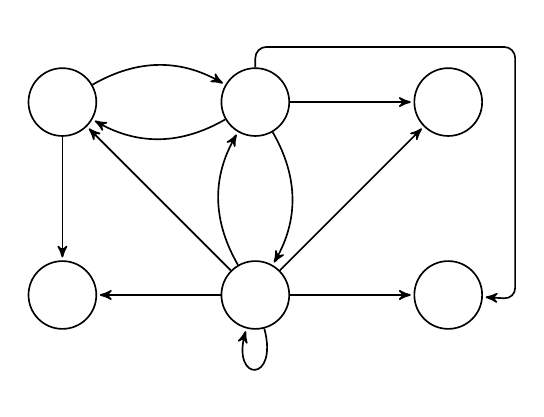
\begin{tikzpicture}[->,>=stealth',shorten >=1pt,auto,node distance=2.5cm,
                    semithick]
  \tikzstyle{every state}=[draw=black,text=black]

  \node[state,inner sep=2pt,scale=0.98]         (A)                    {};
  \node[state,inner sep=2pt,scale=0.98]         (B)       [right of=A] {};
  \node[state,inner sep=2pt,scale=0.98]         (D)       [below of=B] {};
  \node[state,inner sep=2pt,scale=0.98]         (E)       [below of=A] {};
    \node[state,inner sep=2pt,scale=0.98]       (F)       [right of=B] {};
    \node[state,inner sep=2pt,scale=0.98]       (H)       [right of=D] {};

  \path (A) edge [bend left] node {} (B);
  \path (B) edge [bend left] node[swap] {} (A);
\path (B) edge [bend left] node[swap] {} (D);
\path (D) edge node[xshift=2mm] {} (A);
  \path (D) edge [bend left] node {} (B);
   \path (D) edge [loop below] node {} (D);
  \path (A) edge node {} (E);
  \path (B) edge node[swap] {} (F);
\path (D) edge node[swap] {} (H);

\path  (D) edge node {} (E);
\path  (D) edge node[swap,xshift=-2mm] {} (F);
\draw [->,rounded corners] (B) -- ++(0,0.7) -- node {} ++(3.3,0) -- ++(0,-3.2) -- (H);
\end{tikzpicture}
\\
product~
\end{tabular}
\end{center}
\caption{A UBA~, Markov chain , and their product
  , as described in Example~\ref{ex:product}.}
\label{fig:product}
\end{figure}

The following proposition shows that the powers of (submatrices of)  admit a probabilistic interpretation.
Roughly, Proposition~\ref{prop:powers-of-B} states that the entries of the th matrix power are probabilities of length- paths in the Markov chain that trigger certain runs in the automaton.
\begin{proposition} \label{prop:powers-of-B}
Let  and .
Let .
Define  and

Then .
In particular:

\end{proposition}
\begin{proof}
Let  and .
Since the unambiguous automaton~ is diamond-free, it has at most one run for  from  to~.
A sequence  is such a run if and only if .
Such a path is in  if and only if .
In that case we have:

We conclude that, for fixed , the probability of those  for which there are  with   equals .
The proposition follows.
\qed
\end{proof}

\subsection{Recurrent SCCs}
\label{sub:recurrent}
In this section we define a notion of recurrent SCC for the matrix
, generalizing the familiar notion of the same name for finite
Markov chains.  We classify each recurrent SCC  as either accepting
or non-accepting, showing that  is nonzero just in case
 is accepting.

If automaton  is deterministic then the matrix  in
\eqref{eq:basic-eq-2-matrix} is stochastic.  While  need not be
stochastic if  is merely unambiguous, we have
\begin{proposition} \label{prop:spectral-radius-le-1}
  .
\end{proposition}
\begin{proof}
By Proposition~\ref{prop:powers-of-B}, for all , all entries of~ are at most~.
Let  be a dominant eigenvector, i.e., .
Then  is bounded over all~.
It follows that .
\qed
\end{proof}

Using Theorem~\ref{thm:nonnegative}(2), it follows from
Proposition~\ref{prop:spectral-radius-le-1} that for any
 we have .  An SCC
 of  is called \emph{recurrent} if
.  Such an SCC~ is said to be \emph{accepting} if
, i.e., if the collection
of all automaton states in  is an accepting set.

The following lemma summarizes the key properties of recurrent SCCs
that we will need.
\begin{restatable}{lemma}{lemrecurrent}\label{lem:recurrent}\label{LEM:RECURRENT}
  Let  be a recurrent SCC.
\begin{enumerate}
\item We have .
\item For all , we have  iff  is accepting.
\end{enumerate}
\end{restatable}
\noindent Lemma~\ref{lem:recurrent} is proved in Section~\ref{sec:recurrent-proof}.

\begin{example}
Consider the matrix  from Example~\ref{ex:product}, shown in
Figure~\ref{fig:product}.  This matrix has a single recurrent SCC,
namely .
It is accepting, as the automaton uses a B\"uchi acceptance condition.
We have:

The vector  is a dominant eigenvector of .
\end{example}

\subsection{Cuts}
\label{sub:cut}
In this subsection we introduce the notion of a cut of an SCC.
Among other things, this yields a purely graph-theoretic
characterization of recurrent SCCs: an SCC is recurrent just in case
it has a cut.

Let  be an SCC of~.  A set
 is called a \emph{fiber} of  if it can be
written  for some  and
.  Given such a fiber  and , if 
then we define a fiber
 If  then  is undefined.  We extend
this definition inductively by
 and
 for  and
.
We have that  is defined if and only if  describes a path in~.
If  is a singleton~, we may write  for .


  We call a fiber  a \emph{cut} of~ if
  (i)~ for some  and ,
  and (ii)~ holds for all  such that
   is defined.
Clearly if  is a cut then so is  when the
latter is defined.  Given a cut , we call its
characteristic vector  a \emph{cut vector}.

The following lemma summarizes the key properties of cuts that we will need.\begin{restatable}{lemma}{lemcut}\label{lem:cut}\label{LEM:CUT}
Let  be an SCC.  Then
\begin{enumerate}
\item  is recurrent if and only if it has a cut.
\item If  is accepting recurrent and  is a cut vector then .
\item If  is recurrent one can compute a cut in polynomial time.
\end{enumerate}
\end{restatable}
\noindent Lemma~\ref{lem:cut} is proved in Section~\ref{sec:cut-proof}.

Given an accepting recurrent SCC~, say that a vector  is a
\emph{-normalizer} if .  Then
Lemma~\ref{lem:cut}(2) says that a cut vector for  is a
-normalizer.

\begin{example}
  Consider the matrix  from Example~\ref{ex:product}, shown in
  Figure~\ref{fig:product}, and its single recurrent SCC .  Then
   is a cut and
   is another cut.  Both
  the associated cut vectors are -normalizers.
  For  example, let  be the cut vector associated with , i.e., .
  Since , we have .
\end{example}

\subsection{The Augmented Linear System} \label{sub:augmented}
We now extend \eqref{eq:basic-eq-2-matrix} to a linear
system that has  as unique solution.
\begin{lemma} \label{lem:linear-system}
Let  be the set of accepting recurrent SCCs, and  the
set of non-accepting recurrent SCCs.  For each  let
 be a -normalizer (which
exists by Lemma~\ref{lem:cut}(2)).  Then ~is the unique
solution of the following linear system:

\end{lemma}
\begin{proof}
  The vector~ solves~\eqref{eq:linear-system}: indeed, this
  follows from the equality , the definition of a
  -normalizer, and Lemma~\ref{lem:recurrent}(2).

  It remains to show uniqueness.  To this end, let
   solve~\eqref{eq:linear-system}.  We show that
  .
We proceed by induction over the DAG of SCCs of~.
Let  be any SCC (possibly trivial, i.e.,  for some , and ).
Let us write  for the set of SCCs directly below~.
By the induction hypothesis, we have  for all SCCs .
We have to show that .
Since  and , we have


\begin{itemize}
\item
Let  be non-recurrent.
Then we must have , as otherwise, by~\eqref{eq:linear-system-uniqueness}, the vector  would be an eigenvector of~ associated with eigenvalue~, implying , and thus contradicting the assumption that  is not recurrent.
\item
Let  be recurrent. If , then .
Therefore, we can assume that .
By Lemma~\ref{lem:recurrent}(1), .
Thus, with~\eqref{eq:linear-system-uniqueness}, .
By Theorem~\ref{thm:irreducible}(2), the eigenspace of~ associated with the spectral radius is one-dimensional, implying that  is a scalar multiple of~.
We have , hence .
\qed
\end{itemize}
\end{proof}

Now we can prove our main result, Theorem~\ref{thm:PMC-MC-UBA}.
\begin{proof}[of Theorem~\ref{thm:PMC-MC-UBA}]
Given a Markov chain~, an initial distribution~, and a diamond-free unambiguous automaton~, proceed as follows.
\begin{enumerate}
\item Set up the matrix~ from Section~\ref{sub:linear-system}.
\item Compute the SCCs of~.
\item For any SCC , check whether  is recurrent, by seeing if the linear system  has a nonzero solution.
\item For any accepting recurrent SCC~, compute a cut vector  using Lemma~\ref{lem:cut}(3).
\item Solve the linear system~\eqref{eq:linear-system} in Lemma~\ref{lem:linear-system}.
\item Compute  using~\eqref{eq:basic-eq-1} in Lemma~\ref{lem:basic-eq}. \qed
\end{enumerate}
\end{proof}

\section{Proof of Lemma~\ref{lem:recurrent}}
\label{sec:recurrent-proof}

In this section we prove Lemma~\ref{lem:recurrent}, which is restated here.

\lemrecurrent*

\subsection{Proof of Lemma~\ref{lem:recurrent}(1)}
\paragraph{Proof of Lemma~\ref{lem:recurrent}(1)}
Recall that .
Thus, .
Since  and  is strongly connected, it follows, by Theorem~\ref{thm:irreducible}(4), that .  \qed

\subsection{Proof of Lemma~\ref{lem:recurrent}(2)}
The proof of Lemma~\ref{lem:recurrent}(2) requires some auxiliary
definitions and results.

Let  be two SCCs of matrix .  We write
 if  is reachable from~.  Note that
 is a partial order on the SCCs.
In case matrix  is stochastic the recurrent SCCs are just the
bottom SCCs.  While this does not hold in general, we have the
following result.
\begin{proposition}
\label{prop:lower-matrices-zero}
Let  be a recurrent SCC.  Then all SCCs~
are such that .
\end{proposition}
\begin{proof}
Recall that .
Thus,  by Lemma~\ref{lem:recurrent}(1).
Hence, we have for any  that .
So if  then .
It follows that  for
all SCCs  directly below~.
Using the definitions of~ and~ it follows that  must hold for all SCCs~.
\qed
\end{proof}

In the following two propositions we consider paths in~ along with ``corresponding'' paths in~.
The gist of Propositions \ref{prop:recurrent} and~\ref{prop:recurrent-2} is that paths in~ that have ``corresponding'' paths in~ that linger in a strict subset of an SCC are negligible.

Let  and  denote the obvious projection maps.  We extend both
maps pointwise to finite and infinite sequences; e.g., we have .

\begin{proposition}
  Let  be a recurrent SCC, let  be strongly
  connected, and let .  Define  and
  write

Then  iff .
\label{prop:recurrent}
\end{proposition}
\begin{proof}
Let  be a dominant eigenvector of  and write
 and  for the
respective minimum and maximum entries of .  Since 
is strongly connected, by Theorem~\ref{thm:irreducible}(1) and~(2), we have .

Intuitively,  contains those paths in~ that correspond to a path in~.
For  and , recall the notation   from Proposition~\ref{prop:powers-of-B}.
Write also .
Intuitively,  contains those paths in~ that correspond to a path in~ for at least  steps.
Then  by K\H{o}nig's Lemma.
We have for any :


  Suppose now that . Then  and thus

By continuity of measures it follows that .

Conversely, suppose that .  Then

But  by Theorem~\ref{thm:irreducible}(3).
By continuity of measures it follows that .  \qed
\end{proof}

In the following proposition,  includes those infinite paths in~ that correspond to paths in~ that eventually linger in~ for a strict subset~ of an SCC~ in~.
By Proposition~\ref{prop:recurrent} such paths have measure zero.
\begin{proposition}
Let  be a recurrent SCC.
Write

Then  for all .
\label{prop:recurrent-2}
\end{proposition}
\begin{proof}
Let , and , and  be strongly connected, and .
Then  by Proposition~\ref{prop:recurrent}.
Thus  is a countable union of sets of measure zero with respect to~.
It follows .
\qed
\end{proof}


\paragraph{Proof of Lemma~\ref{lem:recurrent}(2)}
Let .
We show that  iff  is accepting.

Suppose that  is accepting.
Recall the definitions of  and~ in Propositions \ref{prop:recurrent} and~\ref{prop:recurrent-2}.
Since  is accepting, we have .
Hence:


Suppose now that  is not accepting.  Let 
be such that .  Since  is not accepting,
 must eventually either remain in a strongly connected set  or reach an SCC .  Thus we have

We have  by Proposition~\ref{prop:recurrent-2}.
For any SCC , , and , we
have
 with the last equality following from
Proposition~\ref{prop:lower-matrices-zero}.  Thus the right-hand side
of \eqref{eq:meas-zero} is a countable union of sets of measure zero
with respect to .  It follows that
.
\qed

\section{Proof of Lemma~\ref{lem:cut}} \label{sec:cut-proof}
In this section we prove Lemma~\ref{lem:cut}, which is restated here.

\lemcut*

\subsection{Proof of Lemma~\ref{lem:cut}(1)}
\paragraph{Proof of Lemma~\ref{lem:cut}(1)}
Let  be an SCC.
We have for all :

Define .
By Theorem~\ref{thm:irreducible}(1),  has a dominant
eigenvector~, positive in all entries, with .  Write  for the smallest entry
of~.  For any  and 
define a random variable  by

We have:

where  denotes expectation with respect to~.

Towards the direction~``'', let  be a cut, where .
Then for all  we have .
So we have for all , using Markov's inequality:

This gives a uniform lower bound on~ for all .
Hence , and so  is recurrent.

Towards the converse~``'', suppose that  has no cuts.
Let .
Since  has no cuts, for any set  there exists  with .
It follows that there are  and  such that for all :

Thus, for all :

Hence,  converges to~ almost surely with respect to~.
Since  is bounded (by ), it follows .
By~\eqref{eq:Ex-X}, we conclude , i.e.,  is not recurrent.
\qed

\subsection{Proof of Lemma~\ref{lem:cut}(2)}
For the proof of Lemma~\ref{lem:cut}(2)  we use the following standard
fact about model checking Markov chains:
\begin{lemma} \label{lem:regular}
Let  be a Markov chain, and  an -regular language.
Suppose  such that .
Then there exists  such that .
\end{lemma}
\begin{proof}[sketch]
Let  be a deterministic Muller automaton that accepts~.
Let  be the initial state of~.
Since , there is a path  in the product of  and~ that leads to a bottom SCC that is non-accepting, i.e., whose corresponding set of automaton states does not satisfy the Muller acceptance condition.
Then  has the required properties.
\qed
\end{proof}

\paragraph{Proof of Lemma~\ref{lem:cut}(2)}

Let  be a recurrent SCC, and let  be a cut.
Recall that  and define .
Since all elements of  are reachable from~ in~, by Proposition~\ref{prop:lower-matrices-zero} we have , thus .
Let  be the cut vector associated with~.
Then we have:

where the last equality holds as the sets  are disjoint by unambiguousness.
Hence .
Suppose .
Then .
Then by Lemma~\ref{lem:regular} there exists  such that

Equivalently,

But since  is a cut, we have , i.e, there exists  with .
By~\eqref{eq:cut=normalizer-proof} we have .
With Lemma~\ref{lem:recurrent}(2) it follows that  is not accepting.
\qed

\subsection{Proof of Lemma~\ref{lem:cut}(3)} \label{sub:computing-cuts}

Let  be a recurrent SCC.
In this section we show how to compute a cut in polynomial time.
By Lemma~\ref{lem:cut}(2), this also yields a -normalizer if  is accepting.

Since automaton  is diamond-free, we have that if  with  then any sets  and~ are disjoint.
\begin{lemma} \label{lem:get-larger}
Let  be a recurrent SCC.
Let .
Suppose  is such that  is not a cut.
Then there are  and  with  and .
Hence .
\end{lemma}
\begin{proof}
Since  is recurrent, by Lemma~\ref{lem:cut}(1),  has a cut~, say .
Since  is an SCC, there is  with , hence  is also a cut.
Again, since  is an SCC, there is  with .
Define .
Then  is a cut.
Moreover, we have .
Since  is a cut but  is not, we have:

So there is  with .
\qed
\end{proof}

\begin{lemma} \label{lem:compute-cut}
Let  be a recurrent SCC.
Let .
The following algorithm is a polynomial-time algorithm that computes  with  such that  is a cut of~:
\begin{enumerate}
\item  (the empty word)
\item while  and  such that  and  \\
\mbox{}\hspace{4mm} 
\item return 
\end{enumerate}
\end{lemma}
\begin{proof}
By Lemma~\ref{lem:get-larger} the algorithm returns a cut.
In every iteration, the set~ increases (cf.~Lemma~\ref{lem:get-larger}), so the algorithm terminates after at most  iterations.

Consider the directed graph~ with

Then for any  and  we have  if and only if there are  such that

is a path in~.
It follows that with a (polynomial-time) reachability analysis of~ one can compute all  for which there exists  with .
The shortest such~ correspond to shortest paths in~, hence satisfy .
Moreover, one can check in polynomial time whether .
\qed
\end{proof}

\section{An NC Model Checking Procedure} \label{sec:NC}

In this section we show that one can model check Markov chains against unambiguous automata in NC.
To achieve this we strengthen our assumptions on the acceptance condition:
we assume that the given automaton  has an NC-decidable acceptance condition; i.e., given~ and a set , one can compute in~NC whether .
This is the case, e.g., if  is given as a B\"uchi condition.
We show:
\begin{theorem} \label{thm:NC}
  Given a Markov chain , an initial distribution~, and an unambiguous automaton~ with NC-decidable acceptance condition,
  the value  is computable in~NC.
\end{theorem}
As a consequence, our approach yields optimal complexity for model checking Markov chains against LTL specifications:
\begin{corollary} \label{cor:LTL-PSPACE} Given a Markov chain ,
  an initial distribution~, and an LTL formula~, the
  value  is computable in PSPACE.
\end{corollary}
\begin{proof}
  There is a classical polynomial-space procedure that
  translates~ into an (exponential-sized) B\"{u}chi automaton
  ~\cite{VardiWolper86}.  As noted by several authors
  (e.g.,~\cite{ChaKat14,CouSahSut03}), this procedure can easily be
  adapted to ensure that  be a UBA.

  Now recall from Section~\ref{sec:prelim} that a function that is
  computable in NC is also computable in poly-logarithmic space. By
  Theorem~\ref{thm:NC} it follows that we can compute
   in poly-logarithmic space in 
  and .  Thus using standard techniques for composing
  space-bounded transducers (see, e.g.,~\cite[Proposition
  8.2]{Pap94}), we can compute  using
  polynomial space in  and . \qed
\end{proof}

Towards a proof of Theorem~\ref{thm:NC}, observe that most steps of
the algorithm from the proof of Theorem~\ref{thm:PMC-MC-UBA} can be
implemented in~NC in a straightforward way.  The exception is the
cut-computation algorithm from Lemma~\ref{lem:compute-cut}, which
seems inherently sequential.  Recall that we used this algorithm
because a cut vector of an accepting recurrent SCC~ yields a
-normalizer (Lemma~\ref{lem:cut}(2)) and we need such a normalizer
to set up up the equation system~\eqref{eq:linear-system} from
Lemma~\ref{lem:linear-system}.  Note that any convex combination of
normalizers is also a normalizer.  In the following we show how to
compute such a normalizer in~NC.

Let  be a recurrent SCC.
Let .
Define .
Observe that  is fibered on~, i.e., there is  with .
For any  and  and  with  we write  to avoid clutter.
Hence

One can compute~ in~NC by a graph reachability analysis.
Similarly, one can compute in~NC for any  a word  such that .
One can also compute in~NC for any  a matrix  such that  if and only if .
Define

In the following, for a set , we write  for the characteristic vector of~. If  is a singleton set~ we may write  for~.
The following lemma provides a -normalizer:
\begin{lemma} \label{lem:A-limit}
Let  be an accepting recurrent SCC.
Let .
Define  and~ as above.
Then the limit

exists.
The vector  with
0.5ex]
    0 & \text{otherwise}
\end{cases}
 \label{eq:then=mult}
  \vec{\chi}(q_0)^\top A(q_1) \cdot \ldots \cdot A(q_n) \ = \ \vec{\chi}(q_0 \then v_{q_1} \cdots v_{q_n})^\top

 \vec{\chi}(q_0)^\top \ \leqslant \ \vec{\chi}(q_0)^\top A \ \leqslant \ \vec{\chi}(q_0)^\top A^2 \ \leqslant \ \cdots

q_0 \ = \ q_0 \then \varepsilon \ \subsetneq \ q_0 \then v_{\bar q_1} \subsetneq \ q_0 \then v_{\bar q_2} v_{\bar q_1} \ \subsetneq \ \ldots \ \subsetneq \ q_0 \then v_{\bar q_k} \cdots v_{\bar q_2} v_{\bar q_1}

\vec{\nu}(\vec{x})_{\<q s\>} =
\begin{cases}
    \vec{x}_{q} & \text{if } q \in R \text{ and } s = s_0 \
By Lemma~\ref{lem:cut}(2) for all  the vector  is a -normalizer, i.e., .
Defining  with , we have  for all .
Note that ~is a linear function.

Consider the stochastic process  where the  are chosen from~ independently and uniformly at random.
Write  and~ for the associated probability measure and expectation.
It follows from~\eqref{eq:then=mult} that we have


In the following, when we say `almost surely' we mean with probability~ with respect to~.
Almost surely,  will eventually appear as a contiguous subsequence of .
That is,  almost surely.
Thus, almost surely there is  such that  holds for all .
Hence,

So we have

i.e.,  is a -normalizer.
\qed
\end{proof}

\begin{lemma} \label{lem:xi}
The vector~ with  from Lemma~\ref{lem:A-limit} is the unique solution of the linear system

where  is a vector of variables indexed by~, and  is the matrix with  if and only if .
\end{lemma}
\begin{proof}
Recall from the proof of Lemma~\ref{lem:A-limit} that we have  for all~.
It follows that  and thus .
Hence we have:

So  solves~\eqref{eq:xi}.
Towards uniqueness, since

we have:

Since  holds for all , it follows that  is less than~ in all entries.
Hence .
Let  be any solution of~\eqref{eq:xi}.
Then .
Since , it follows .
\qed
\end{proof}

Now we can prove Theorem~\ref{thm:NC}.
\begin{proof}[of Theorem~\ref{thm:NC}]
We follow the same approach as in the proof of Theorem~\ref{thm:PMC-MC-UBA}.
Most steps can easily be carried out in~NC.
Instead of step~4, we compute, in~NC \cite[Theorem~5]{BorodinGathenHopcroft82}, the vector~ by solving the linear system~\eqref{eq:xi} in Lemma~\ref{lem:xi}.
From~ we easily obtain a -normalizer by Lemma~\ref{lem:A-limit}.
\qed
\end{proof}



\section{Implementation and Experiments}
\label{uba_implementation}



We implemented a probabilistic model checking procedure for Markov chains
and UBA specifications using the algorithm detailed in Section~\ref{sec:uba}
as an extension to the probabilistic model checker
\prism{}~\cite{prism40} version 4.4 beta.
\footnote{More details are available
    at~\url{https://wwwtcs.inf.tu-dresden.de/ALGI/TR/JCSS19/}.
}
All experiments were carried out on a computer with
 two
 Intel E5-2680 8-core CPUs at 2.70~GHz with  of RAM running Linux, a time
 limit of  minutes and a memory limit of .
Our implementation is based on the \explicitengine{} engine of \prism{}, where
the Markov chain is represented explicitly.
Our implementation supports UBA-based model checking for handling the
LTL fragment of \prism's -like specification language
as well as direct verification against a path specification given by a
UBA provided in the HOA format~\cite{Hanoi-CAV15}. For LTL formulas,
we rely on external LTL-to-UBA translators.
For the purpose of the benchmarks
we employ the \ltltotgba{} tool from \spot{}~\cite{Duret14} version 2.7
to generate a UBA for a given LTL formula.
For the linear algebra parts of the algorithms, we use the \colt{}
library~\cite{Hoschek04}.

\subsection{Analyzing SCCs}
In our experiments we solved the linear system~\eqref{eq:linear-system} SCC-wise, bottom-up.
We call accepting recurrent SCCs \emph{positive}.
We considered two different variants for checking positivity of an SCC.
The first variant relies on \colt{} to perform a QR
decomposition of the matrix for the SCC to compute the rank, which allows for
deciding the positivity of the SCC.
The second approach
is based on a variant of the power iteration
method for iteratively computing an eigenvector.

\paragraph{Recurrence check via rank computation}
\label{sec:rank}

Let  be an SCC.
Using Theorem~\ref{thm:nonnegative}(1) we can check whether  is recurrent by seeing if the linear system  has a nonzero solution.
It is equivalent to check whether the matrix  has full rank, where  is the  identity matrix.
Indeed, if  has full rank, then it has a trivial kernel , so  does not have a nonzero solution.
Conversely, if  does not have full rank, then there is a nonzero  with .


\paragraph{Iterative algorithm}

Consider again an SCC , and define .
Denote by  the column vector all whose components are~.
For  define .
Our algorithm is as follows.
Exploiting the recurrence  compute the sequence
 until we find  with either  (by this inequality we mean strict inequality in all components)
or .
In the first case we conclude that  is not recurrent. 

In the second case we conclude that  is recurrent.
If  is, in addition, accepting, then we can use the result of our iterative computation to simplify the linear system~\eqref{eq:linear-system}:
we compute a cut vector  and a scalar  so that , and replace all equations in~\eqref{eq:linear-system} with variables from  on the left-hand side by .
This algorithm is justified by the following two lemmas, combined with Lemma~\ref{lem:cut}(2).

\begin{lemma} \label{lem-iter-zero-new}
 is recurrent if and only if there is no  with
    .
\end{lemma}

\begin{lemma} \label{lem-iter-pos-new}
If  is recurrent, then  exists, and , and
     is a scalar multiple of .
\end{lemma}

For the proofs we need the following two auxiliary lemmas:
\begin{lemma} \label{lem-iter-aux-new}
    For any  and any  we have  if
    and only if .
    In particular,  and~ have the same eigenvectors with eigenvalue~.
\end{lemma}
\begin{proof}
Immediate.
\qed
\end{proof}

\begin{lemma} \label{lem-iter-matrix-conv-new}
Let  denote the spectral radius of~.
Then the matrix limit  exists and is strictly positive in all entries.
\end{lemma}
\begin{proof}
Since  is irreducible,  is strictly positive (in all entries).
By Theorem~\ref{thm:irreducible}(5) the matrix limit
 
 exists and is strictly positive.
\qed
\end{proof}

\begin{proof}[of Lemma~\ref{lem-iter-zero-new}]
Let  with .
It follows from Theorem~\ref{thm:irreducible}(4) that the spectral radius of~ is .
Hence by Lemma~\ref{lem-iter-aux-new} the spectral radius of~ is also , i.e.,  is not recurrent.

For the converse, suppose  is not recurrent, i.e., the spectral radius of~ is .
Let  denote the spectral radius of~.
By Lemma~\ref{lem-iter-aux-new}, we have .
If  then  is the zero matrix and we have .
Let .
It follows from Lemma~\ref{lem-iter-matrix-conv-new} that there is  such
that  (with the inequality strict in all components).
Hence  and .
\qed
\end{proof}

\begin{proof}[of Lemma~\ref{lem-iter-pos-new}]
Let  be recurrent, i.e., the spectral radius of~ is~.
So, with Lemma~\ref{lem-iter-aux-new} the spectral radius of~ is~.
By Lemma~\ref{lem-iter-matrix-conv-new} the limit  exists and is positive.
From the definition of  we have .
By Lemma~\ref{lem-iter-aux-new} also .
Lemma~\ref{lem:recurrent}(1) states .
By Theorem~\ref{thm:irreducible}(2), the eigenspace
of~ associated with the spectral radius is one-dimensional, implying that  is a scalar multiple of~.
\qed
\end{proof}

In our implementation we replace the check whether  by a check whether  and~ are approximately equal, up to a convergence threshold of .
Thus, our implementation is sound only up to these numerical issues.

\subsection{Evaluation of the rank computation}

\label{sec:appendix-experiments}
\label{appendix:experiments}

The iterative (power iteration) algorithm from the previous subsection has the benefit that, in addition to deciding positivity of an SCC,
the computed eigenvector can be directly used to compute
the values of  corresponding to a positive SCC, once a cut has been found.
We have evaluated the performance and scalability of
the cut generation algorithm together with both approaches for
treating SCCs with selected automata specifications
that are challenging for our UBA-based model checking approach. 


\begin{figure}[t]
    \hspace*{-0.97 em}
    \scalebox{0.97}{\begin{tikzpicture}[initial text=,initial where=left, every node/.style={thick}, every path/.style={thick}]
        \node[state, initial, accepting, ellipse, minimum size=2 em, inner sep=0 em]    (q)     at(0,0) {};
        \coordinate                 (coord)             at(0,-0.2625 \textwidth) {};

        \foreach \line in {1,...,4}
        {
            \foreach \column in {1,...,3}
            {
                \node[state, ellipse, minimum size=2 em, inner sep=0 em] (q\column\line) at () {};
            }
            \draw[->]   (q1\line) edge[]  node[above] {} (q2\line);
        }
        \draw[->]   (q)     edge[]  node[left, pos=0.75]  {}   (q11);
        \draw[->]   (q)     edge[]  node[below, pos=0.62] {}    (q12);
        \draw[->]   (q)     edge[]  node[above, pos=0.62, yshift=-0.5 ex] {}    (q13);
        \draw[->]   (q)     edge[]  node[left, pos=0.75]  {}   (q14);
        \draw[->]   (q21)   edge[]  node[above] {}     (q31);
        \draw[->]   (q22)   edge[]  node[above] {}     (q32);
        \draw[->]   (q23)   edge[]  node[above] {}     (q33);
        \draw[->]   (q24)   edge[]  node[above] {}     (q34);

        \draw[->] plot [smooth] coordinates {() () () (0.35 em, 1.05 em)};
        \node[draw=none]    (symb0) at()  {};
        \draw[->] plot [smooth] coordinates {() () () (0.85 em, 0.62 em)};
        \node[draw=none]    (symb2) at()  {};
        \draw[->] plot [smooth] coordinates {() ()  (1.05 em, 0 em)};
        \node[draw=none]    (symb3) at()  {};
        \draw[->] plot [smooth] coordinates {() () () ()};
        \node[draw=none]    (symb1) at()  {};
    \end{tikzpicture}\begin{tikzpicture}[initial text=,initial where=left, every node/.style={thick}, every path/.style={thick}]
        \node[state, initial, accepting, ellipse, minimum size=2 em, inner sep=0 em]    (q)     at(0,0) {};
        \coordinate                 (coord)             at(0,-0.2625 \textwidth) {};

        \foreach \line in {1,...,4}
        {
            \foreach \column in {1,...,3}
            {
                \node[state, ellipse, minimum size=2 em, inner sep=0 em] (q\column\line) at () {};
            }
            \draw[->]   (q1\line) edge[]  node[above] {} (q2\line);
        }
        \draw[->]   (q)     edge[]  node[left, pos=0.75]  {}   (q11);
        \draw[->]   (q)     edge[]  node[below, pos=0.62] {}    (q12);
        \draw[->]   (q)     edge[]  node[above, pos=0.62, yshift=-0.5 ex] {}    (q13);
        \draw[->]   (q)     edge[]  node[left, pos=0.75]  {}   (q14);
        \draw[->]   (q21)   edge[]  node[above] {}     (q31);
        \draw[->]   (q22)   edge[]  node[above] {}     (q32);
        \draw[->]   (q23)   edge[]  node[above] {}     (q33);
        \draw[->]   (q24)   edge[]  node[above] {}     (q34);

        \draw[->]       (q34)   edge[loop right]    node[right] {} (q34);
        \draw[->] plot [smooth] coordinates {() () () (0.85 em, 0.62 em)};
        \node[draw=none]    (symb2) at()  {};
        \draw[->] plot [smooth] coordinates {() ()  (1.05 em, 0 em)};
        \node[draw=none]    (symb3) at()  {};
        \draw[->] plot [smooth] coordinates {() () () ()};
        \node[draw=none]    (symb1) at()  {};
    \end{tikzpicture}}
\caption{UBA ``complete automaton'' (left) and ``nearly complete automaton''
(right) for .}
\label{fig:uba-complete-nearly-complete}
\end{figure}


To assess the scalability of our implementation in the face of
particularly difficult UBA, we considered two families of
parametrized UBA. Both have an alphabet defined over a single atomic
proposition resulting in a two-element alphabet that we use to
represent either a  (meaning the negated atomic proposition) or a  bit
(meaning the positive atomic proposition). The first automaton
(``complete automaton''),
depicted in Figure~\ref{fig:uba-complete-nearly-complete} on the left for ,
is a complete automaton, i.e.,
recognizes . It consists of a single,
accepting starting state that nondeterministically branches to one
of  states, each one leading after a further step
to a -state chain that only lets a particular -bit bit-string
pass, subsequently returning to the initial state. As all the -bit
bit-strings that can occur have a chain, the automaton is
complete. Likewise, the automaton is unambiguous as each of the
bit-strings can only pass via one of the chains.

Our second automaton (``nearly complete automaton''),
depicted in Figure~\ref{fig:uba-complete-nearly-complete} on the right for ,
arises from the first automaton by a modification of the
chain for the ``all zero'' bit-string, preventing the return to the
initial state. Clearly, the automaton is not complete.

We use both kinds of automata in an experiment using our extension of
\prism{} against a simple, two-state DTMC that encodes a uniform
distribution between the two ``bits''. This allows us to determine
whether the given automaton is almost universal. As the \prism{}
implementation requires the explicit specification of a DTMC, we end
up with a product that is slightly larger than the UBA, even though we
are essentially performing the UBA computations for the uniform
probability distribution.
In particular, this
experiment serves to investigate the scalability of our implementation
in practice for determining whether an SCC is positive, for the cut
generation and for computing .
It should be noted that equivalent deterministic automata, e.g.,
obtained by determinizing the UBA using the \ltltodstar{} tool, are significantly
smaller (in the range of tens of states) due to the fact that the UBA
in question are constructed inefficiently on purpose.

Table~\ref{tab:bench-complete-automaton} presents statistics for
our experiments with the ``complete automaton'' with various parameter
values , resulting in increasing sizes of the UBA and the SCC
(number of states). We list the time spent for generating a cut
(), the number of iterations in the cut generation algorithm of
Lemma~\ref{lem:compute-cut}, and the size of the
cut. In all cases, the cut generation requires 2 iterations. Then we
compare the SCC handling based on power iteration with the SCC
handling relying on a rank computation for determining positivity of
the SCC and a subsequent computation of the values. For the power
iteration method, we provide the time spent for iteratively computing
an eigenvector () and the number of iterations
(iter.).
For the other method, we provide the time spent for the positivity
check by a rank computation with a QR decomposition from the \colt{}
library () and for the subsequent computation of
the values via solving the linear equation system
(). We used an overall timeout of 60 minutes for
each \prism{} invocation and an epsilon value of  as the
convergence threshold.

As can be seen, the power iteration method for the numeric SCC
handling performs well, with a modest increase in the number of
iterations for rising~ until converging on an
eigenvector, as it can fully exploit the sparseness of the matrix.
The QR decomposition for rank computation
performs worse. The time for cut generation exhibits a super-linear
relation with , which is reflected in the larger number of words
that were checked to determine that they are an extension. Note that
our example was chosen in particular to put stress on the cut
generation.

The results for the ``nearly complete automaton'', shown in
Table~\ref{tab:bench-nearly-complete-automaton}, focus on the
computation in the ``dominant SCC'', i.e., the one containing all the
chains that return to the initial state. For the other SCC,
containing the self-loop, non-positivity is immediately clear as it
does not contain a final state. In contrast to the ``complete
automaton'', no cut generation takes place, as the SCC is not
positive. The results roughly mirror the ones for the ``complete
automata'', i.e., the power iteration method is quite efficient in
determining that the SCC is not positive, while the QR decomposition
for the rank computation needs significantly more time and scales
worse.

As the power iteration method performed better, our benchmark results
presented in the following subsections use this method for the SCC handling.


\begin{landscape}
\begin{table}[tbp]
\centering
\begin{tabular}{r|r|r|r|r|r|r|r|r|r}
  &
  &
  & \multicolumn{3}{c|}{cut generation}
  & \multicolumn{2}{c|}{power iter.}
  & \multicolumn{2}{c}{rank-based}
  \\
   
 & \,
 & \,SCC size
 & 
 & \,ext.\ checks
 & \,cut size
 & \,
 & iter.
 & \,
 & \,
\\ \hline
5
 & 193
 & 258
 & \psec{0.061}
 & 10124
 & 32
 & \subpointone & 215
 & \psec{0.451}
 & \psec{0.368}
 \\

6
 & 449
 & 578
 & \psec{0.123}
 & 40717
 & 64
 & \subpointone & 282
 & \psec{4.329}
 & \psec{4.329}
 \\

7
 & 1025
 & 1282
 & \psec{0.876}
 & 172102
 & 128
 & \psec{0.07}
 & 358
 & \psec{56.517}
 & \psec{56.862}
 \\

8
 & 2305
 & 2818
 & \psec{1.818}
 & 929413
 & 256
 & \psec{0.088}
 & 443
 & \psec{830.796}
 & \psec{835.121}
 \\


9
 & 5121
 & 6146
 & \,\psec{17.919}
 & 6818124
 & 512
 & \psec{0.142}
 & 537
 & -\ \
 & -\ \
 \\
\end{tabular}
\caption{Benchmark results for ``complete automaton''
         with parameter .  stands for time-out.}
\label{tab:bench-complete-automaton}
\end{table}

\begin{table}[btp]
\centering
\begin{tabular}{r|r|r|r|r|r}
  &
  &
  & \multicolumn{2}{c|}{power iteration}
  & \multicolumn{1}{c}{rank-based}
  \\
   
 & \ 
 & \ SCC size
 & \ 
 & \ iter.
 & \ 
\\ \hline
5
 & 193
 & 250
 & \subpointone & 52
 & \psec{0.399}
 \\

6
 & 449
 & 569
 & \subpointone & 78
 & \psec{4.105}
 \\

7
 & 1025
 & 1272
 & \subpointone & 112
 & \psec{54.435}
 \\

8
 & 2305
 & 2807
 & \psec{0.072}
 & 155
 & \psec{844.016}
 \\


9
 & 5121
 & 6134
 & \psec{0.112}
 & 205
 & -\ \
 \\
\end{tabular}
\caption{Benchmark results for ``nearly complete automaton''
         with parameter }
\label{tab:bench-nearly-complete-automaton}
\end{table}

\end{landscape}











\subsection{Case Study: Bounded Retransmission Protocol}

Next we report on benchmarks using the bounded retransmission protocol (BRP)
case study of the \prism{} benchmark suite~\cite{prismBenchmark}.  The model
from the benchmark suite covers a single message transmission, retrying for a
bounded number of times in case of an error. In this protocol the message is
split into several so-called hunks. The number of hunks and the number of
allowed retransmissions are parameters in the model. We set the number of hunks
to  and the maximal of retransmissions to .

We have slightly modified the model
to allow the transmission of an infinite number of messages by restarting the
protocol once a message has been successfully delivered or the bound for
retransmissions has been reached.  We include benchmarks with pre-generated
automata, as well as benchmarks with LTL as starting point.
We include also the
evaluation for deterministic Rabin automata generated by \rabinizer{} from \cite{KMSZ18}.



\paragraph{Automata based specifications}
We consider the property ``the message was retransmitted  steps before an
acknowledgment.''
To remove the effect of selecting specific tools for the LTL to automaton
translation (\ltltotgba{} for UBA, the Java-based \prism{}
reimplementation of \ltltodstar{}~\cite{KB06} to obtain a
deterministic Rabin automaton (DRA) for the \prism{} standard approach),
we first consider model checking directly against automata specifications.
As the language of the property is equivalent to the UBA depicted in
Figure~\ref{fig:uba-examples} (on the left) where
 stands for a retransmission,  for an acknowledgment, and  for
no acknowledgment, we use this automaton and the minimal DBA for
the language (this case is denoted by ). We additionally consider
the UBA and DBA obtained by replacing the self-loop in the last state with a
switch back to the initial state (denoted by ), i.e., roughly applying
the -operator to .






\begin{landscape}
\begin{table}[t]
    \centering
\begin{tabular}{r||r|r|r||r|r|r|r}

   &
   \multicolumn{3}{c||}{\prism{} standard} &
   \multicolumn{4}{c}{\prism{} UBA}\\


   &
    &
    &
    &
    &
    &
    &
   \\\hline
,  &
\pnodes{33} &
\pnodes{61025} &
\psec{0.442} &
\pnodes{6} &
\pnodes{34118} &
\psec{0.251} &
\\
 &
\pnodes{33} &
\pnodes{75026} &
\psec{0.398} &
\pnodes{6} &
\pnodes{68474} &
\psec{1.348} &
\psec{1.022}
\\\hline
,  &
\pnodes{129} &
\pnodes{62428} &
\psec{0.481} &
\pnodes{8} &
\pnodes{36164} &
\psec{0.249} &
\\
 &
\pnodes{129} &
\pnodes{97754} &
\psec{0.499} &
\pnodes{8} &
\pnodes{99460} &
\psec{1.71} &
\psec{1.325}
\\\hline
,  &
\pnodes{513} &
\pnodes{64715} &
\psec{0.619} &
\pnodes{10} &
\pnodes{38207} &
\psec{0.261} &
\\
 &
\pnodes{513} &
\pnodes{134943} &
\psec{0.713} &
\pnodes{10} &
\pnodes{136427} &
\psec{2.595} &
\psec{2.11}
\\\hline
,  &
\pnodes{32769} &
\pnodes{83845} &
\psec{4.162} &
\pnodes{16} &
\pnodes{44340} &
\psec{0.31} &
\\
 &
\pnodes{32769} &
\pnodes{444653} &
\psec{4.879} &
\pnodes{16} &
\pnodes{246346} &
\psec{6.817} &
\psec{6.078}
\\\hline
,  &
\pnodes{131073} &
 &
 &
\pnodes{18} &
\pnodes{46390} &
\psec{0.322} &
\\
 &
\pnodes{131037} &
 &
 &
\pnodes{18} &
\pnodes{282699} &
\psec{8.885} &
\psec{7.96}
\\\hline
,  &
 &
 &
 &
\pnodes{50} &
\pnodes{79206} &
\psec{0.825} &
\\
 &
 &
 &
 &
\pnodes{50} &
\pnodes{843414} &
\psec{72.432} &
\psec{70.286}
\end{tabular}
    \caption{Statistics for DBA/DRA- and UBA-based model checking of
      the BRP case study, a
      DTMC with  states,
showing the number of
      states for the automata and the product
      and the time for model checking ().
For , the time for checking positivity ()
      is included in .
The mark  stands for ``not available'' or timeout (30 minutes).}
    \label{table:brp-aut}
\end{table}
\end{landscape}


Table \ref{table:brp-aut} shows results for selected  (with a timeout of  minutes),
demonstrating that for this case study and properties
our UBA-based implementation is generally competitive with the
standard approach of \prism{} based on deterministic automata.
For , our implementation detects that the UBA has a
special shape where all final states have a true-self loop which
allows skipping the SCC handling.
If we execute the positivity check nevertheless,  is in the sub-second range for all considered .
At a certain point, the implementation of the standard approach in
\prism{} becomes unsuccessful, due to \prism{} size
limitations in the product construction of the Markov chain and the
deterministic automaton
(/: ).
As can be seen, using the UBA approach
we can scale the parameter  beyond 
when dealing directly with the automata-based specifications
(/) and within reasonable time required for model checking.


\paragraph{LTL based specifications}

We consider two LTL properties: The first one is:

where  stands for .
The formula~
ensures that  steps before an acknowledgment the message was retransmitted.
Hence, it is equivalent to the property described by the automaton~.
For the LTL-to-automaton translation we
included the Java-based \prism{} reimplementation of \ltltodstar{}
\cite{KB06} to obtain a deterministic Rabin automaton (DRA) for the \prism{} standard approach as well as the tool \rabinizer{} (version 3.1) from \cite{EsparzaKS16}. For the
generation of UBA, we relied on \spot{} (version 2.7), as it is
the only tool that is capable of generating UBA explicitly. 
\begin{landscape}
\begin{table}[tbp]
\centering
\begin{tabular}{r||r|r|r||r|r|r||r|r|r}
   k
   &
   \multicolumn{3}{c||}{\prism{} standard} &
   \multicolumn{3}{c||}{\prism{} \rabinizer} &
   \multicolumn{3}{c}{\prism{} UBA}\\
    
    
   &
    &
    &
    &
    &
    & 
    &
    &
    & 
   
   \\\hline
 & \pnodes{122} & \pnodes{62162} & \psec{1.678} & \pnodes{18} & \pnodes{60642} & \psec{0.568} & \pnodes{6} & \pnodes{34118} & \psec{0.628} \\\hline
 & \pnodes{4602} & \pnodes{72313} & \psec{3.336} & \pnodes{66} & \pnodes{61790} & \psec{0.641} & \pnodes{8} & \pnodes{36164} & \psec{0.534} \\\hline
 &  &  &  & \pnodes{258} & \pnodes{63698} & \psec{1.049} & \pnodes{10} & \pnodes{38207} & \psec{0.568} \\\hline
 &  &  &  & \pnodes{1026} & \pnodes{66739} & \psec{3.754} & \pnodes{12} & \pnodes{40249} & \psec{0.672} \\\hline
 &  &  &  & \pnodes{4098} & \pnodes{71660} & \psec{38.514} & \pnodes{14} & \pnodes{42293} & \psec{1.006} \\\hline
 &  &  &  & \pnodes{16386} & \pnodes{79576} & \psec{925.455} & \pnodes{16} & \pnodes{44340} & \psec{5.837} \\\hline
 &  &  &  &  &  &  & \pnodes{18} & \pnodes{46390} & \psec{132.873} \end{tabular}
\caption{Statistics for automata-based (standard, \rabinizer{}, and UBA)
    model checking of the BRP model and . For every approach the
    corresponding automata sizes and product sizes are depicted.
     The overall model
    checking times ( are listed, which includes the time for
    automata translation.}
\label{table:brp-ltl1}
\end{table}

\begin{table}[btp]
\centering
\begin{tabular}{r||r|r|r||r|r|r||r|r|r|r|r}
   k
   &
   \multicolumn{3}{c||}{\prism{} standard} &
   \multicolumn{3}{c||}{\prism{} \rabinizer} &
   \multicolumn{5}{c}{\prism{} UBA}\\
    
    
   &
    &
    &
    &
    &
    & 
    &
    &
    & 
    &
    &
   
   \\\hline
 & \pnodes{6} & \pnodes{29358} & \psec{0.682} & \pnodes{5} & \pnodes{29358} & \psec{0.435} & \pnodes{4} & \pnodes{31422} & \subpointone & n/a & \psec{0.315} \\\hline
 & \pnodes{17} & \pnodes{37678} & \psec{0.945} & \pnodes{7} & \pnodes{35630} & \psec{0.507} & \pnodes{8} & \pnodes{41822} & \psec{4.84} & \psec{0.192} & \psec{5.435} \\\hline
 & \pnodes{65} & \pnodes{39726} & \psec{1.117} & \pnodes{11} & \pnodes{37678} & \psec{0.537} & \pnodes{14} & \pnodes{45934} & \psec{5.151} & \psec{0.204} & \psec{5.78} \\\hline
 & \pnodes{314} & \pnodes{43806} & \psec{1.523} & \pnodes{23} & \pnodes{41758} & \psec{0.624} & \pnodes{22} & \pnodes{54126} & \psec{5.785} & \psec{0.287} & \psec{6.565} \\\hline
 & \pnodes{1443} & \pnodes{47902} & \psec{2.329} & \pnodes{59} & \pnodes{45854} & \psec{0.894} & \pnodes{32} & \pnodes{62334} & \psec{6.523} & \psec{0.255} & \psec{7.29} \\\hline
 & \pnodes{9016} & \pnodes{56029} & \psec{5.273} & \pnodes{167} & \pnodes{53997} & \psec{2.097} & \pnodes{44} & \pnodes{78669} & \psec{9.484} & \psec{0.214} & \psec{10.294} \\\hline
 & \pnodes{67964} &  &  & \pnodes{491} & \pnodes{58081} & \psec{9.579} & \pnodes{58} & \pnodes{86853} & \psec{10.351} & \psec{0.214} & \psec{11.307} \\\hline
 &  &  &  & \pnodes{1463} & \pnodes{66217} & \psec{76.115} & \pnodes{74} & \pnodes{103157} & \psec{13.852} & \psec{0.266} & \psec{14.984} \\\hline
 &  &  &  & \pnodes{4379} & \pnodes{70291} & \psec{783.666} & \pnodes{92} & \pnodes{111321} & \psec{15.23} & \psec{0.284} & \psec{16.786} \\\hline
 &  &  &  &  &  &  & \pnodes{112} & \pnodes{127562} & \psec{20.095} & \psec{0.301} & \psec{22.707} \end{tabular}\caption{Statistics for automata-based (standard, \rabinizer{}, and UBA) of the BRP
model and . The structure of this table corresponds to
Table~\ref{table:brp-ltl1}, but with additional listing of the time for the
positivity checks  and cut calculation time
. n/a means not available.}
\label{table:brp-ltl2}
\end{table}
\end{landscape}

Table~\ref{table:brp-ltl1} lists the results for model checking .
From a certain point on, the implementation of the standard approach in \prism{}
is unsuccessful, due to \prism's restrictions in the DRA construction
(). Concerning automata sizes and model checking times, \spot{}
shows the best behavior among \prism{} standard and \rabinizer{}.  \spot{}
actually generates a UFA for  which is recognized by our
implementation and handled as explained in \cite{BenLenWor14}.  The sizes of the
unambiguous automata output by \spot{} grow linearly in , whereas the
sizes of the deterministic automata output by \rabinizer{} grow
exponentially. Thus, \prism{} with \rabinizer{} times out after 
minutes for .  However, \spot{} produces for  an
exponential-sized intermediate automaton, which is then shrunk via
bisimulation to an automaton of linear size. Thus, our implementation \prism{}
UBA times out for .




As a second formula we investigate



where  denotes . This formula requires that every request (sending a message and waiting for an
acknowledgment) is eventually responded to by an answer (the receiver of the
message sends an acknowledgment and this acknowledgment is received within the
next  steps).

Table~\ref{table:brp-ltl2} summarizes the results of the benchmark for
.  Here, the \prism{} standard approach with its own implementation of
\ltltodstar{} finishes the calculations until . The sizes of
the DRA produced by {\prism}'s \ltltodstar{} increase rapidly with~.
For , \prism{} standard can construct the DRA (with
\pnodes{67964} states and within  seconds), but cannot construct
the product anymore.  Similarly, the sizes of the DRA produced by \rabinizer{}
grow rapidly in . The sizes of the DRA of \rabinizer{} are smaller than the
size of the UBA for .

In contrast to the deterministic automata, the UBA sizes increase moderately with~.
In the UBA approach the positivity check is the most time
consuming part of the calculation, whereas the cut generation is always below
 seconds. For  there is no positive SCC, so the
cut calculation is omitted. The model checking process consumes more time
in the UBA case in comparison with \prism{} standard until , but for
bigger  the performance turns around. Even if \prism{} standard were to
complete the calculation for , it would be slower, as the creation
of the DRA takes  seconds. Similarly, \prism{} \rabinizer{} outperforms
\prism{} UBA for , which is due to the time-consuming positivity
check. For bigger , both \prism{} standard and \prism{} \rabinizer{} cannot
finish their calculation within the given time bound, whereas \prism{} UBA
finishes the calculations for all tested . 



\subsection{NBA versus UBA}
\label{sec:nbavsuba}

To gain some understanding of the cost of requiring unambiguity for an
NBA, we compare the sizes of NBA and UBA generated by the
\ltltotgba{} tool of \spot{} for the formulas
of~\cite{EH00,SomBloem00,DwyerAC99}, which have been used for benchmarking, e.g.,
in~\cite{KB06}. We consider both the ``normal'' formulas and their
negations, yielding 188 formulas.


\begin{table}[htbp]
     \centering
     \resizebox{\textwidth}{!}{\begin{tabular}{@{}r|r|r|r|r|r|r|r|r|r}
        Number of states & & & & & & & & & \\\hline
        \ltltotgba{} NBA &  &  &  &  &  &  &  &  & \\
        \ltltotgba{} UBA &  &  &  &  &  &  &  &  & 
     \end{tabular}}
\caption{Number of formulas where the (standard) NBA and UBA has a number
     of states .}
     \label{table:nbavsuba}
 \end{table}

As can be seen in Table~\ref{table:nbavsuba}, both the NBA and UBA are of reasonable size.
Most of the generated UBA () have the same size as the NBA and
for  of the formulas the UBA is at most twice the size
as the corresponding NBA. The largest UBA has 112 states, the second
largest has 45 states.







 
\section{Conclusion}
\label{sec:conclusion}

We have presented a polynomial-time algorithm for Markov chain
analysis against properties given as unambiguous automata.  The
algorithm is based on the analysis of nonnegative matrices and
exploits in particular their spectral theory.

As LTL formulas can be transformed into UBA with a single exponential
blow-up, our algorithm yields a procedure for model checking LTL
formulas on Markov chains that is singly exponential in the formula
size.  We have moreover refined the process of UBA generation and
Markov chain analysis to achieve the optimal PSPACE upper bound for
computing the exact probability that a given Markov chain satisfies a
given LTL formula.



We have developed an extension of \prism{} that supports our approach.
Its experimental evaluation shows that the UBA-based method is very
competitive with the approach using deterministic automata,
outperforming the latter in certain cases.

For the other singly exponential approaches to LTL model checking,
such as using separated automata~\cite{CouSahSut03} or weak
alternating automata~\cite{BusRubVar04}, we are not aware of any
available implementation to compare our approach against.\footnote{The paper \cite{CouSahSut03} addresses experiments with a
  prototype implementation, but this implementation seems not to be
  available anymore.  } Our algorithm for arbitrary UBA can be seen as
a generalization of the approach of~\cite{CouSahSut03}, which requires
separated UBA~\cite{MuellerThesis18}.

Markov chain analysis via general UBA, rather than separated UBA or
deterministic automata, offers additional flexibility that can be
exploited when building automata from LTL formulas.  In particular, it
facilitates use of state-reduction techniques, such as simulation,
that may not preserve the seperatedness property.  As our experiments
(specifically with the bounded retransmission protocol) suggest, the
eigenvalue algorithm can deduce non-positiveness of an SCC very
efficiently in practice.  For the generation of UBA we have used the
tool \spot, which implements a simple and straightforward way to
produce unambiguous B\"uchi automata \cite{DuretHabil17}.
Alternatively, \texttt{Tulip} contains an LTL-to-UBA translator; but
this tool is not available anymore.  As with the approach using
deterministic automata, the performance of the UBA-based method
depends strongly on the availability of small UBA. In contrast to
nondeterministic or deterministic automata, the generation of small
UBA and their simplification has not yet been explored thoroughly.

\bibliographystyle{plain}
\bibliography{lit}


\end{document}
